\documentclass[aspectratio=169]{beamer}

\usepackage[spanish,es-nodecimaldot]{babel}
\usepackage[T1]{fontenc}
\usepackage[utf8]{inputenc}
\usepackage{lmodern}
\usepackage{graphicx}
\usepackage{booktabs}
\usepackage{tabularx}
\usepackage{array}
\usepackage{ragged2e}
\usepackage{xcolor}
\usepackage{hyperref}
\usepackage{tikz}

\usetikzlibrary{arrows.meta,positioning,shapes.geometric}

\usetheme{Madrid}
\usecolortheme{default}
\setbeamertemplate{navigation symbols}{}
\setbeamertemplate{footline}[frame number]

\definecolor{cibblue}{HTML}{0F4C81}
\definecolor{cibteal}{HTML}{1F7A8C}
\definecolor{cibgold}{HTML}{D9A441}

\setbeamercolor{structure}{fg=cibblue}
\setbeamercolor{frametitle}{fg=white,bg=cibblue}
\setbeamercolor{title}{fg=white,bg=cibblue}
\setbeamercolor{block title}{fg=white,bg=cibteal}
\setbeamercolor{block body}{bg=black!3}

\tikzset{
  box/.style={draw=cibblue, rounded corners, fill=cibblue!8, minimum width=2.1cm, minimum height=0.95cm, align=center, font=\small},
  smallbox/.style={draw=cibteal, rounded corners, fill=cibteal!8, minimum width=1.8cm, minimum height=0.8cm, align=center, font=\scriptsize},
  line/.style={-{Latex[length=2mm]}, thick, draw=cibblue}
}

\title{Procesamiento de Flujos de Datos en Tiempo Real a Gran Escala}
\subtitle{Capitulo 4 de \textit{huawei-2022.pdf}}
\author{Jhunior Eduardo Guevara Lázaro}
\institute{Grupo 6 \\ Aprendizaje de Máquina y Minería de Datos}
\date{Docente: Mg. Ing. Yury Tello Canchapoma \\ Lima - Perú, 2026}

\begin{document}

\begin{frame}
  \titlepage
  \vspace{-0.7cm}
  \begin{center}
    
\includegraphics[width=1.6cm]{uni.png}
  \end{center}
\end{frame}

\begin{frame}{Ruta de la exposicion}
  \tableofcontents
\end{frame}

\section{Introduccion}

\begin{frame}{Problema y motivacion}
  \begin{itemize}
    \item Algunos datos pierden valor casi inmediatamente despues de que ocurre el evento.
    \item En fraude, monitoreo, IoT o ciberseguridad, responder tarde equivale a perder la oportunidad de actuar.
    \item El capitulo 4 plantea que el problema no es solo almacenar datos, sino convertirlos en decision operativa con baja latencia.
  \end{itemize}
  \vspace{0.2cm}
  \begin{block}{Idea central}
    El \textit{stream processing} procesa datos en movimiento para producir respuestas utiles en segundos o milisegundos.
  \end{block}
\end{frame}

\begin{frame}{Objetivo del tema}
  \begin{columns}[T]
    \column{0.52\textwidth}
      \textbf{Lo que buscamos entender}
      \begin{itemize}
        \item por que el tiempo cambia el valor del dato;
        \item como se organiza una arquitectura de procesamiento continuo;
        \item que rol cumplen Flume, Kafka, Flink, Structured Streaming y Redis;
        \item como todo esto se aplica a casos reales.
      \end{itemize}
    \column{0.48\textwidth}
      \textbf{Producto final del trabajo}
      \begin{itemize}
        \item monografia;
        \item presentacion;
        \item laboratorio con implementacion en codigo.
      \end{itemize}
  \end{columns}
\end{frame}

\section{Procesamiento en Tiempo Real}

\begin{frame}[plain]
  \centering
  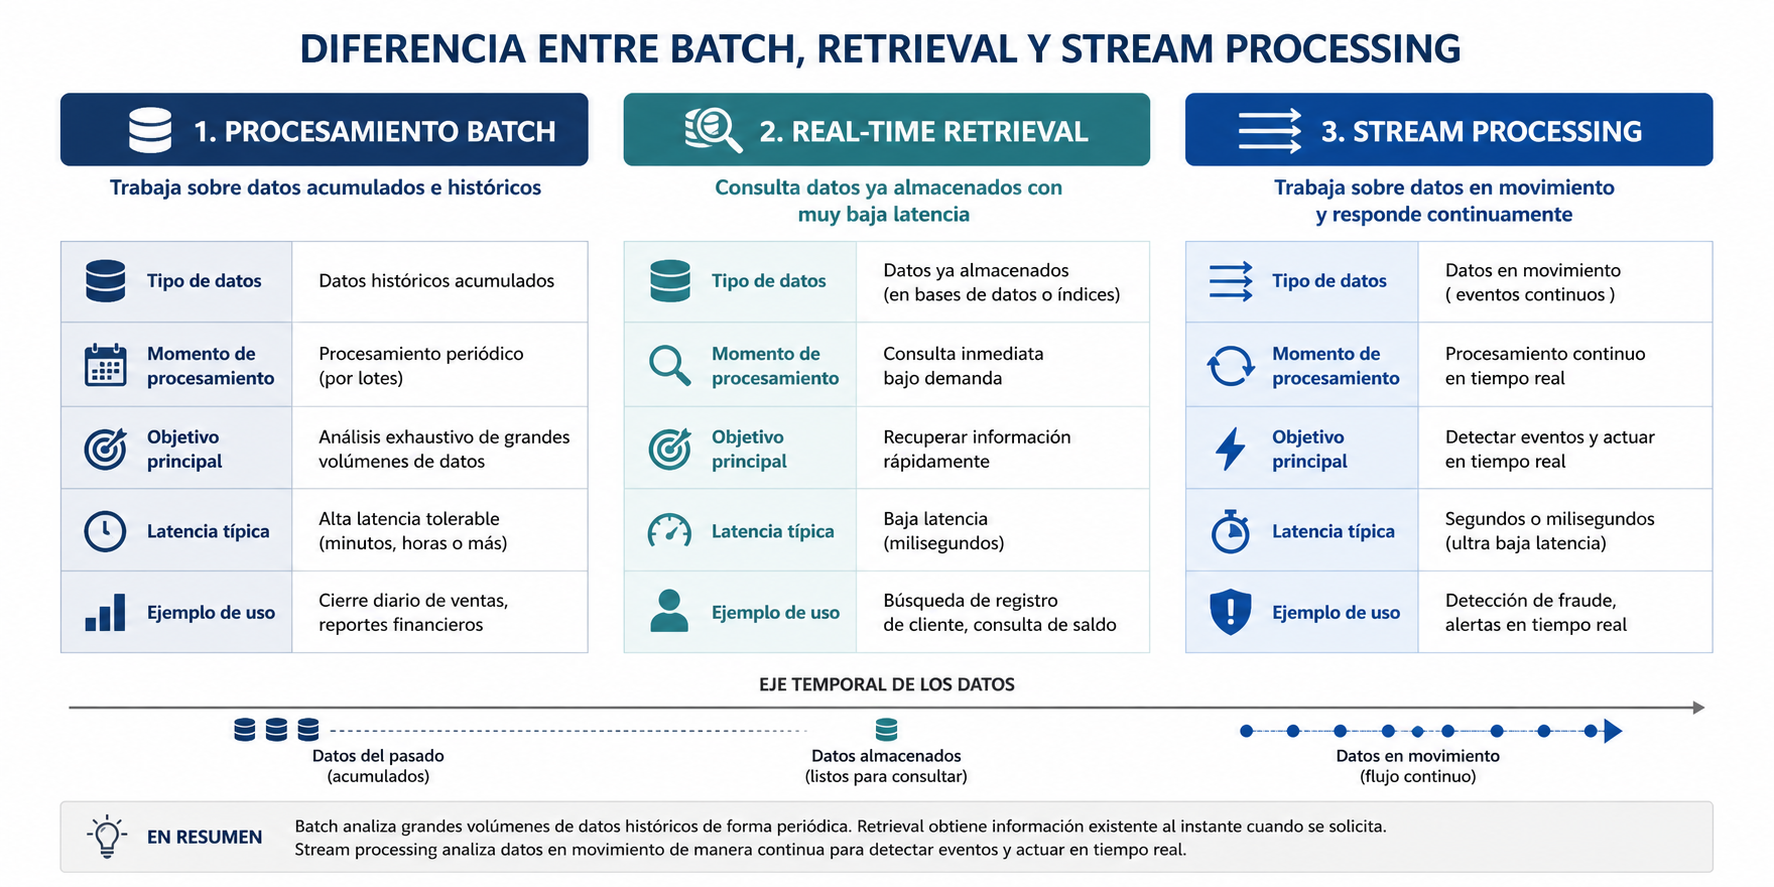
\includegraphics[width=\paperwidth,height=0.9\paperheight,keepaspectratio]{img/01.png}
\end{frame}

\begin{frame}{Lectura del esquema comparativo}
  \begin{itemize}
    \item \textbf{Batch}: analiza datos historicos acumulados.
    \item \textbf{Real-time retrieval}: consulta rapidamente datos ya almacenados.
    \item \textbf{Stream processing}: analiza eventos continuos y reacciona mientras el dato sigue siendo relevante.
    \item La diferencia clave es que el streaming trabaja sobre datos en movimiento, no sobre conjuntos ya cerrados.
  \end{itemize}
\end{frame}

\begin{frame}{Requisitos de una plataforma a gran escala}
  \small
  \begin{tabularx}{\textwidth}{>{\RaggedRight\arraybackslash}p{3.35cm}X}
    \toprule
    \textbf{Requisito} & \textbf{Implicancia} \\
    \midrule
    Baja latencia & Responder en segundos o milisegundos \\
    Alto throughput & Absorber grandes volumenes de eventos \\
    Alta confiabilidad & Evitar perdida, omision y duplicacion no controlada \\
    Escalabilidad horizontal & Crecer agregando nodos al cluster \\
    Multiples fuentes & Integrar logs, BD, APIs, archivos, sensores e IoT \\
    Integracion externa & Enviar resultados a dashboards, caches o motores de reglas \\
    \bottomrule
  \end{tabularx}
\end{frame}

\section{Marco Conceptual}

\begin{frame}[plain]
  \centering
  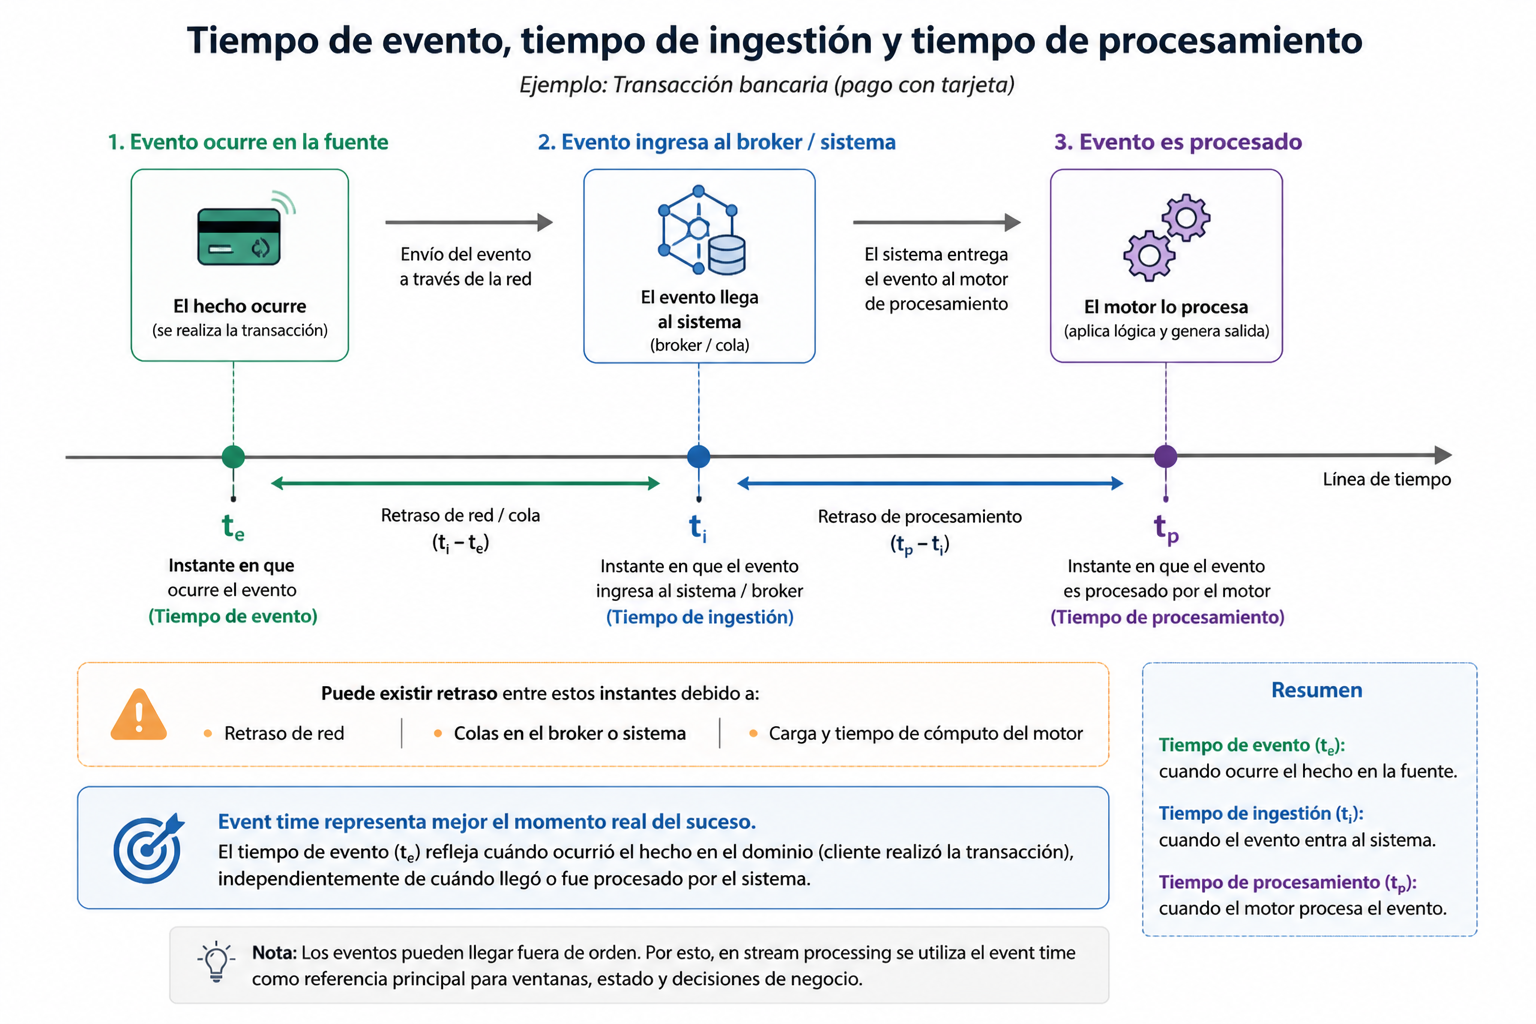
\includegraphics[width=\paperwidth,height=0.9\paperheight,keepaspectratio]{img/02.png}
\end{frame}

\begin{frame}{Idea clave sobre el tiempo}
  \begin{block}{Lectura}
    El evento puede ocurrir en un momento, ingresar al sistema despues y procesarse aun mas tarde.
  \end{block}
  \begin{itemize}
    \item \textbf{Event time}: cuando el hecho ocurrio realmente.
    \item \textbf{Ingestion time}: cuando entra al broker o al sistema.
    \item \textbf{Processing time}: cuando el motor lo procesa.
    \item Para analitica mas fiel suele preferirse el \textit{event time}.
  \end{itemize}
\end{frame}

\begin{frame}[plain]
  \centering
  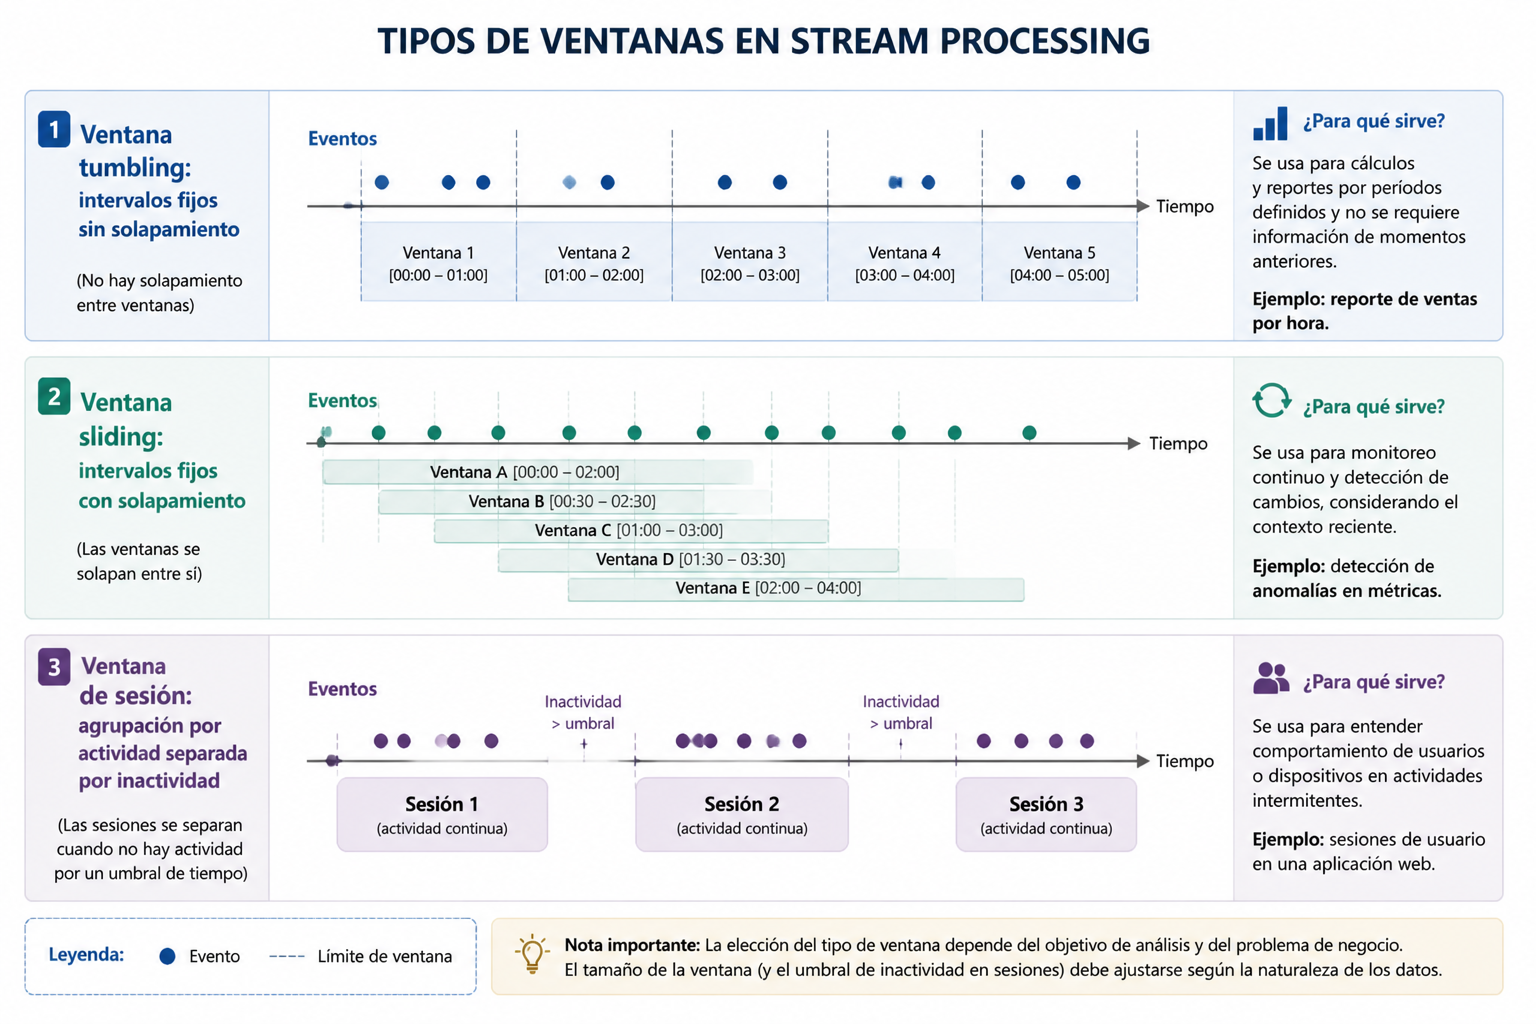
\includegraphics[width=\paperwidth,height=0.9\paperheight,keepaspectratio]{img/03.png}
\end{frame}

\begin{frame}{Lectura de las ventanas}
  \begin{itemize}
    \item \textbf{Tumbling}: intervalos fijos sin solapamiento.
    \item \textbf{Sliding}: intervalos fijos con solapamiento.
    \item \textbf{Session}: agrupacion por actividad separada por inactividad.
    \item Las ventanas permiten agregar un flujo infinito en periodos manejables.
  \end{itemize}
\end{frame}

\begin{frame}{Estado, checkpoints y recuperacion}
  \begin{columns}[T]
    \column{0.58\textwidth}
      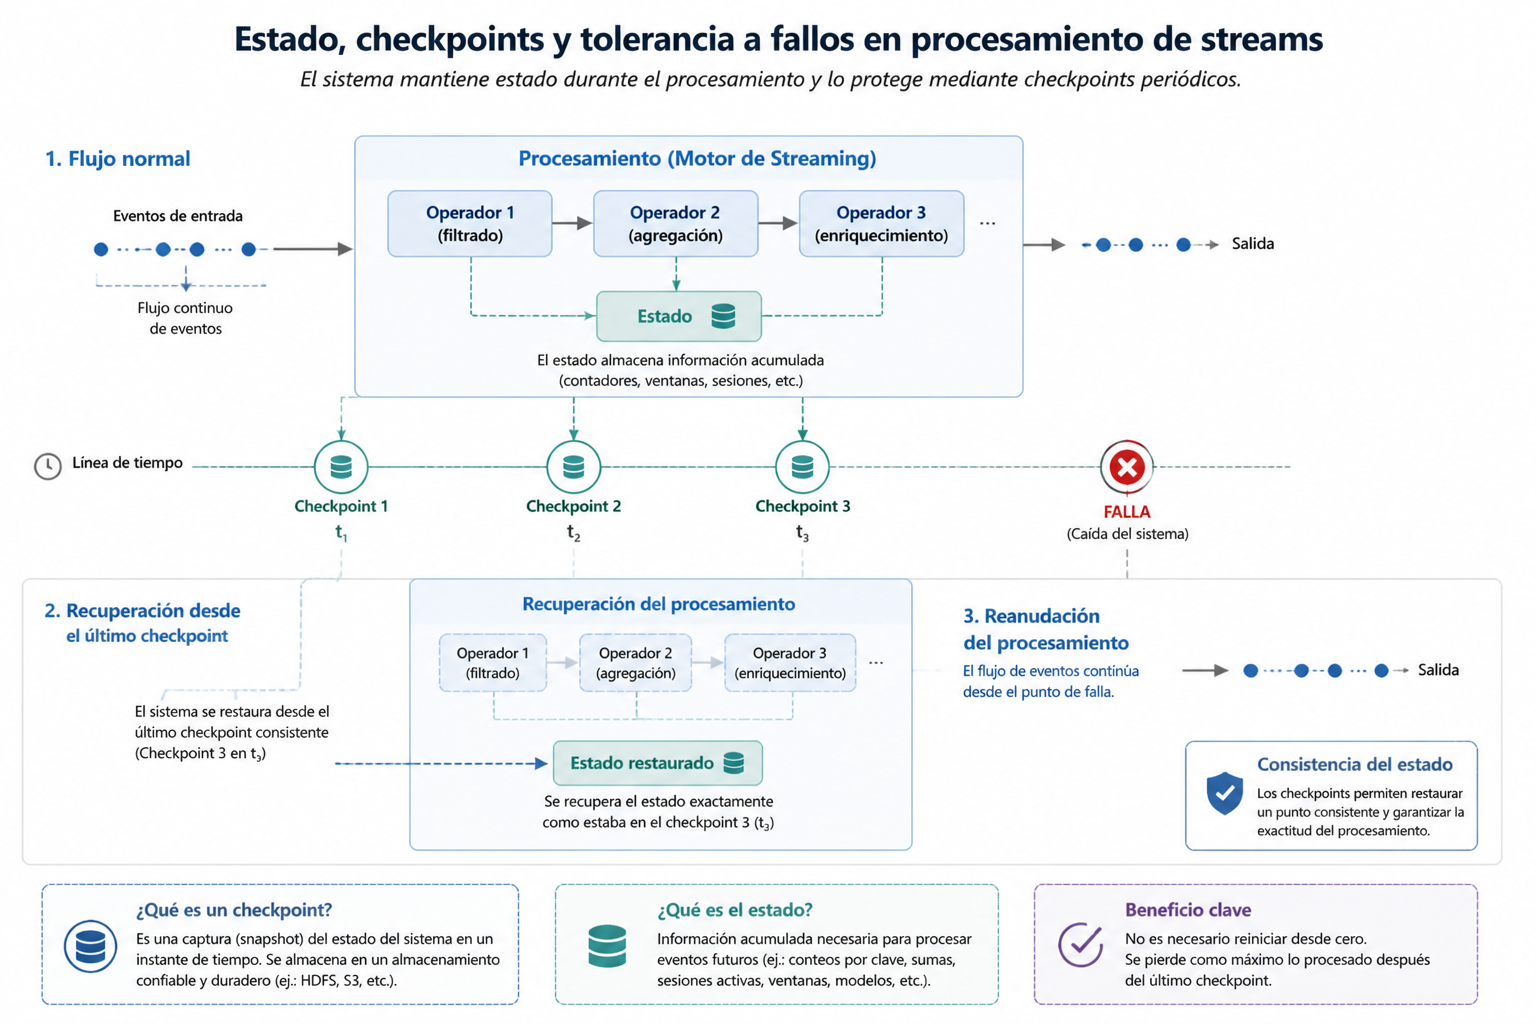
\includegraphics[width=\textwidth]{img/04.png}
    \column{0.42\textwidth}
      \begin{itemize}
        \item Muchas operaciones de streaming son \textit{stateful}.
        \item El estado guarda acumulados, conteos o contexto por clave.
        \item Los \textit{checkpoints} permiten restaurar un punto consistente ante fallos.
      \end{itemize}
      \begin{block}{Clave}
        La tolerancia a fallos no consiste solo en reiniciar, sino en reanudar sin perder consistencia.
      \end{block}
  \end{columns}
\end{frame}

\begin{frame}{Eventos tardios y watermarks}
  \begin{columns}[T]
    \column{0.58\textwidth}
      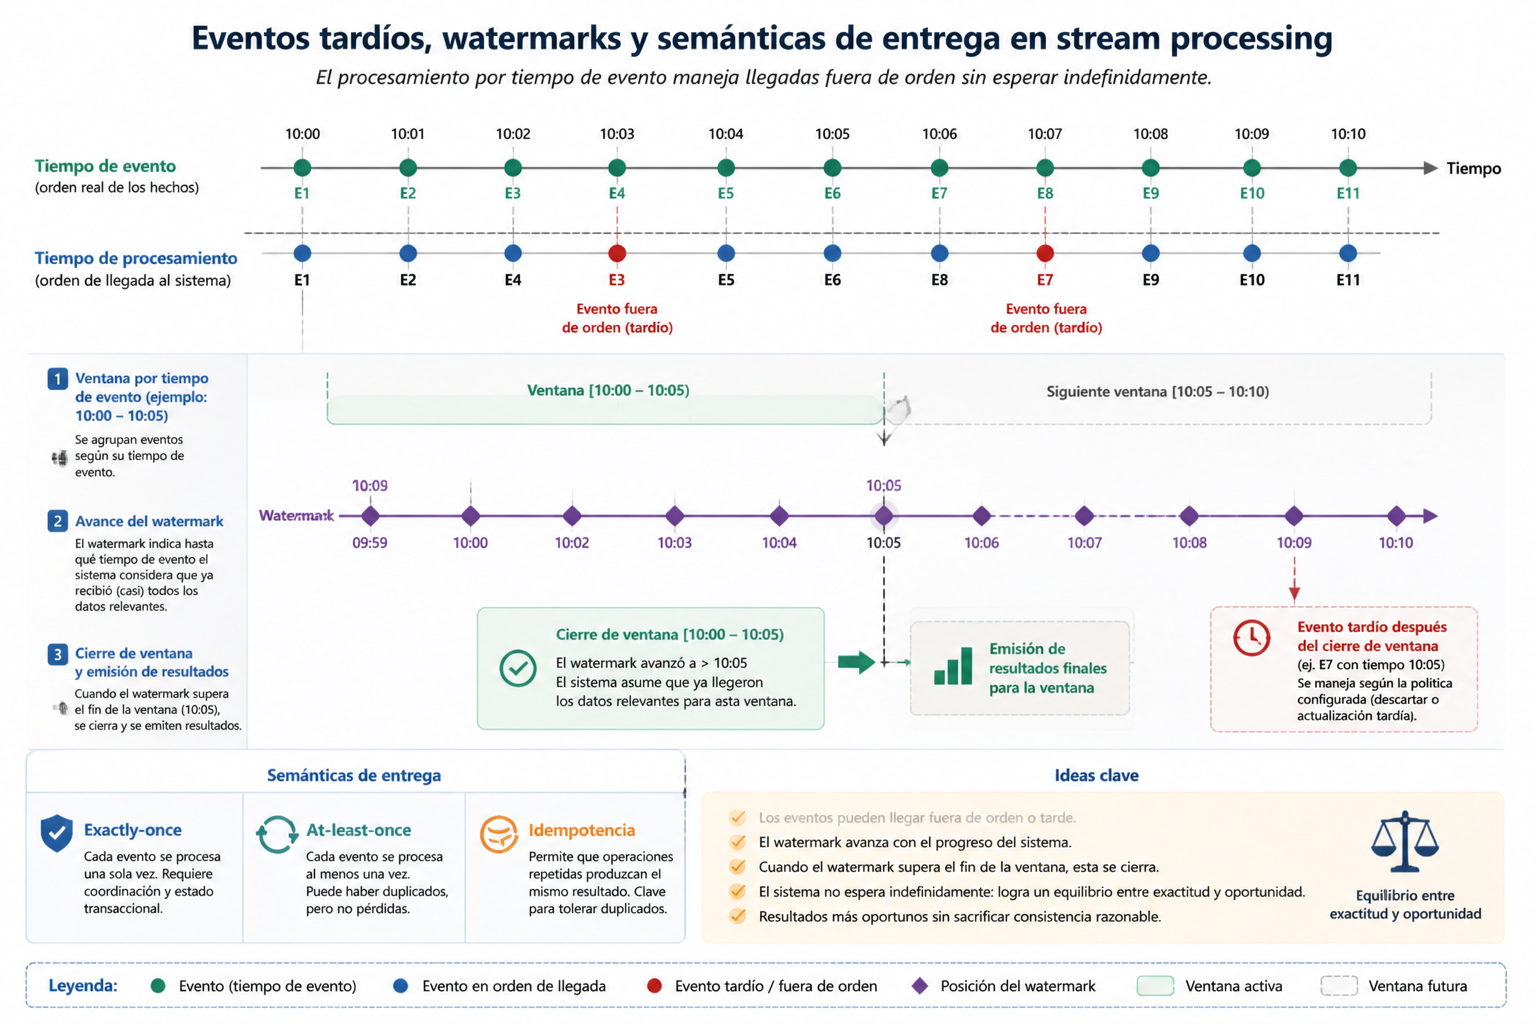
\includegraphics[width=\textwidth]{img/05.png}
    \column{0.42\textwidth}
      \begin{itemize}
        \item Los eventos no siempre llegan en el orden en que ocurrieron.
        \item Los \textit{watermarks} indican hasta donde es razonable esperar datos anteriores.
        \item Esto permite cerrar ventanas sin esperar indefinidamente.
      \end{itemize}
      \begin{block}{Semanticas}
        \textit{At-least-once} acepta duplicados; \textit{exactly-once} busca que cada evento impacte una sola vez.
      \end{block}
  \end{columns}
\end{frame}

\section{Arquitectura}

\begin{frame}[plain]
  \centering
  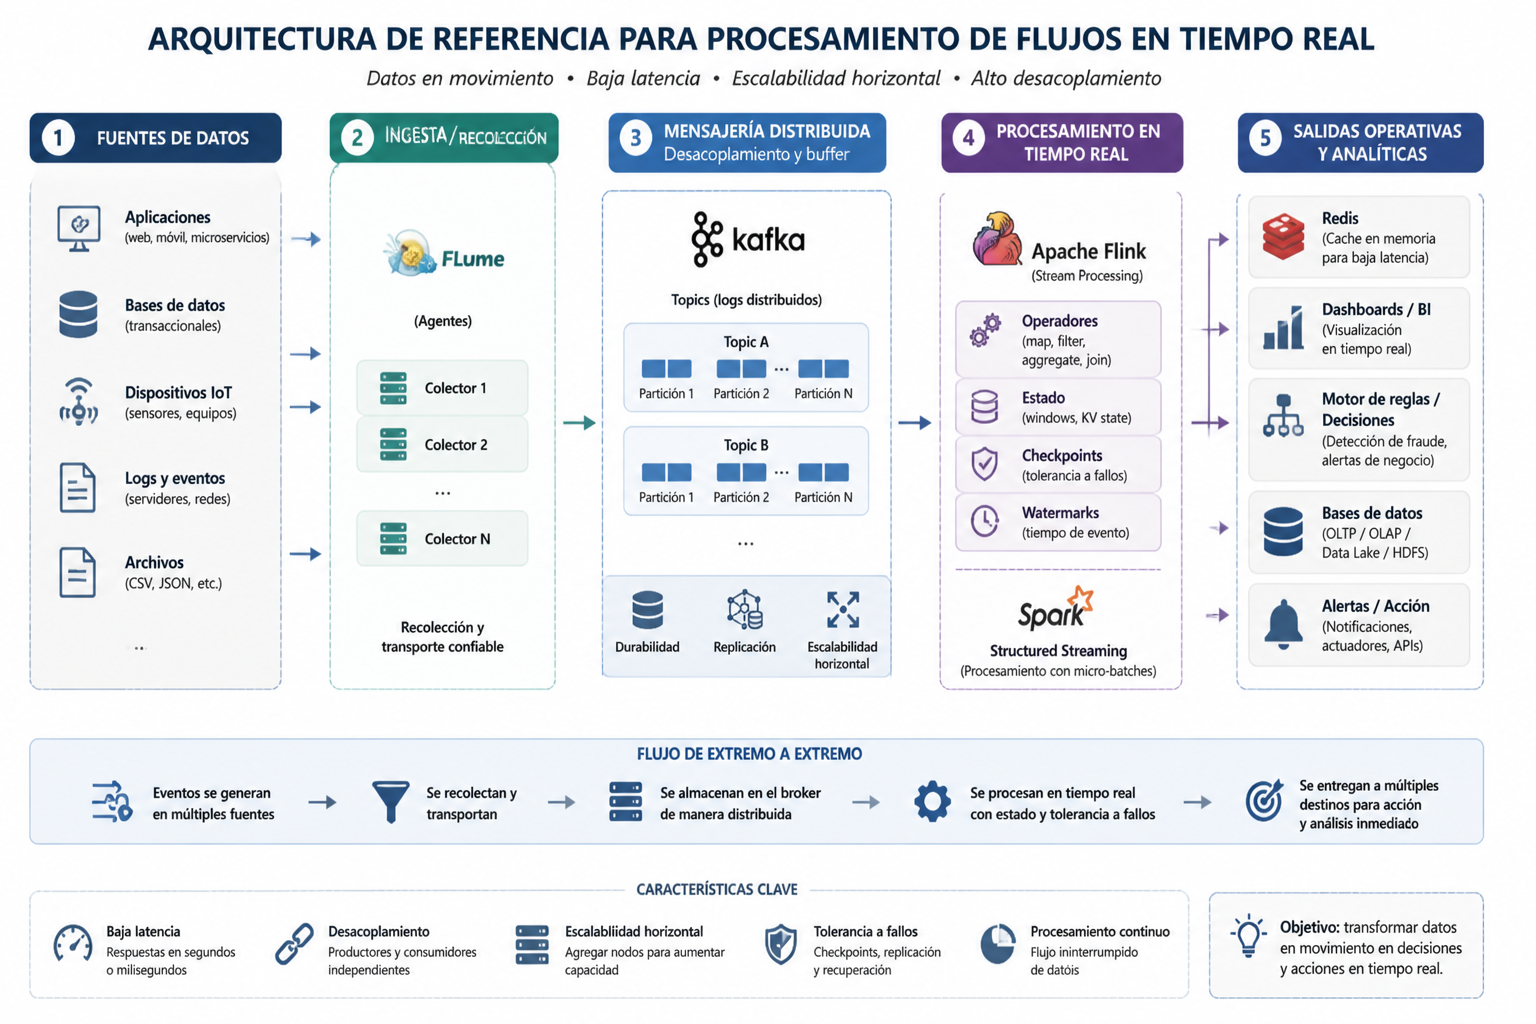
\includegraphics[width=\paperwidth,height=0.9\paperheight,keepaspectratio]{img/06.png}
\end{frame}

\begin{frame}{Lectura de la arquitectura}
  \begin{itemize}
    \item Fuentes heterogeneas alimentan una capa de ingesta.
    \item Kafka desacopla productores y consumidores y absorbe picos de carga.
    \item Flink o Structured Streaming ejecutan la logica de negocio.
    \item Redis, dashboards o motores de reglas consumen la salida y convierten datos en accion.
  \end{itemize}
\end{frame}

\begin{frame}{Flujo funcional del sistema}
  \begin{enumerate}
    \item Se generan eventos desde aplicaciones, bases de datos, sensores o logs.
    \item La capa de ingesta recoge y normaliza la informacion.
    \item El broker distribuye el flujo y absorbe picos de carga.
    \item El motor de procesamiento ejecuta reglas, agregaciones y correlaciones.
    \item La salida se convierte en accion, alerta, visualizacion o consulta rapida.
  \end{enumerate}
\end{frame}

\section{Tecnologias}

\begin{frame}{Tecnologias principales del capitulo}
  \begin{itemize}
    \item \textbf{Flume}: recoleccion y transporte confiable de eventos.
    \item \textbf{Kafka}: bus distribuido para mensajeria y desacoplamiento.
    \item \textbf{Flink}: procesamiento continuo con estado, ventanas y baja latencia.
    \item \textbf{Structured Streaming}: motor de streaming sobre Spark SQL.
    \item \textbf{Redis}: cache y almacenamiento de respuesta rapida.
  \end{itemize}
\end{frame}

\begin{frame}{Flume}
  \begin{columns}[T]
    \column{0.56\textwidth}
      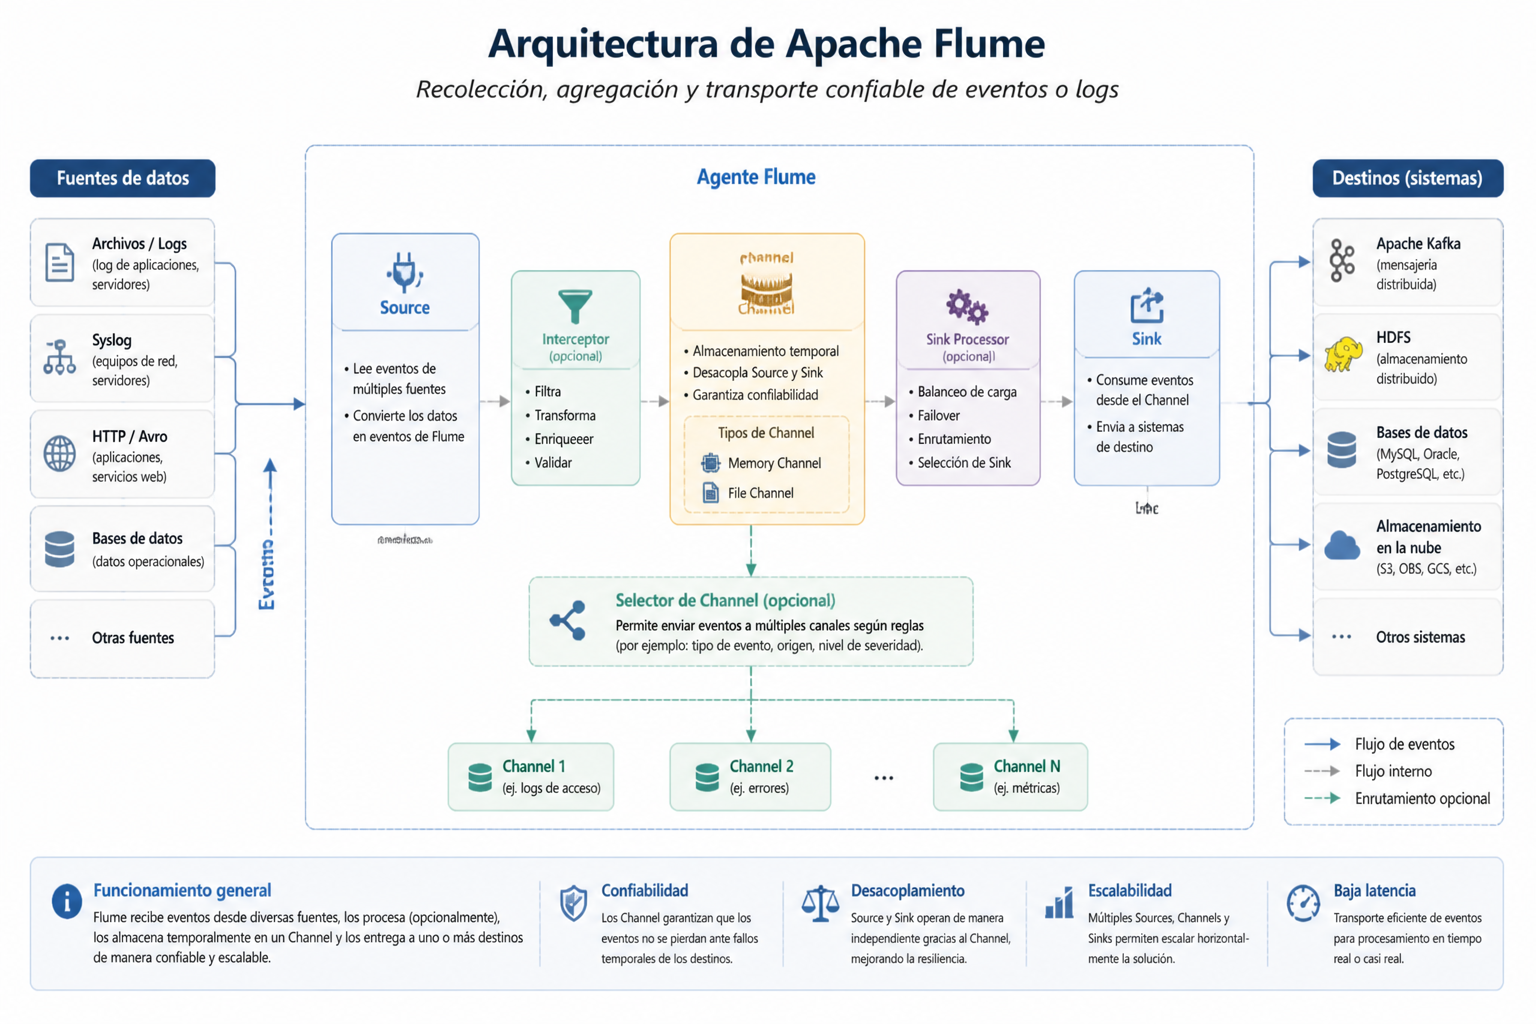
\includegraphics[width=\textwidth]{img/07.png}
    \column{0.44\textwidth}
      \begin{itemize}
        \item Arquitectura base: \textbf{Source -> Channel -> Sink}.
        \item Recoge logs y eventos desde distintas fuentes.
        \item Puede enrutar, enriquecer y reenviar datos al resto del pipeline.
      \end{itemize}
  \end{columns}
\end{frame}

\begin{frame}{Kafka}
  \begin{columns}[T]
    \column{0.56\textwidth}
      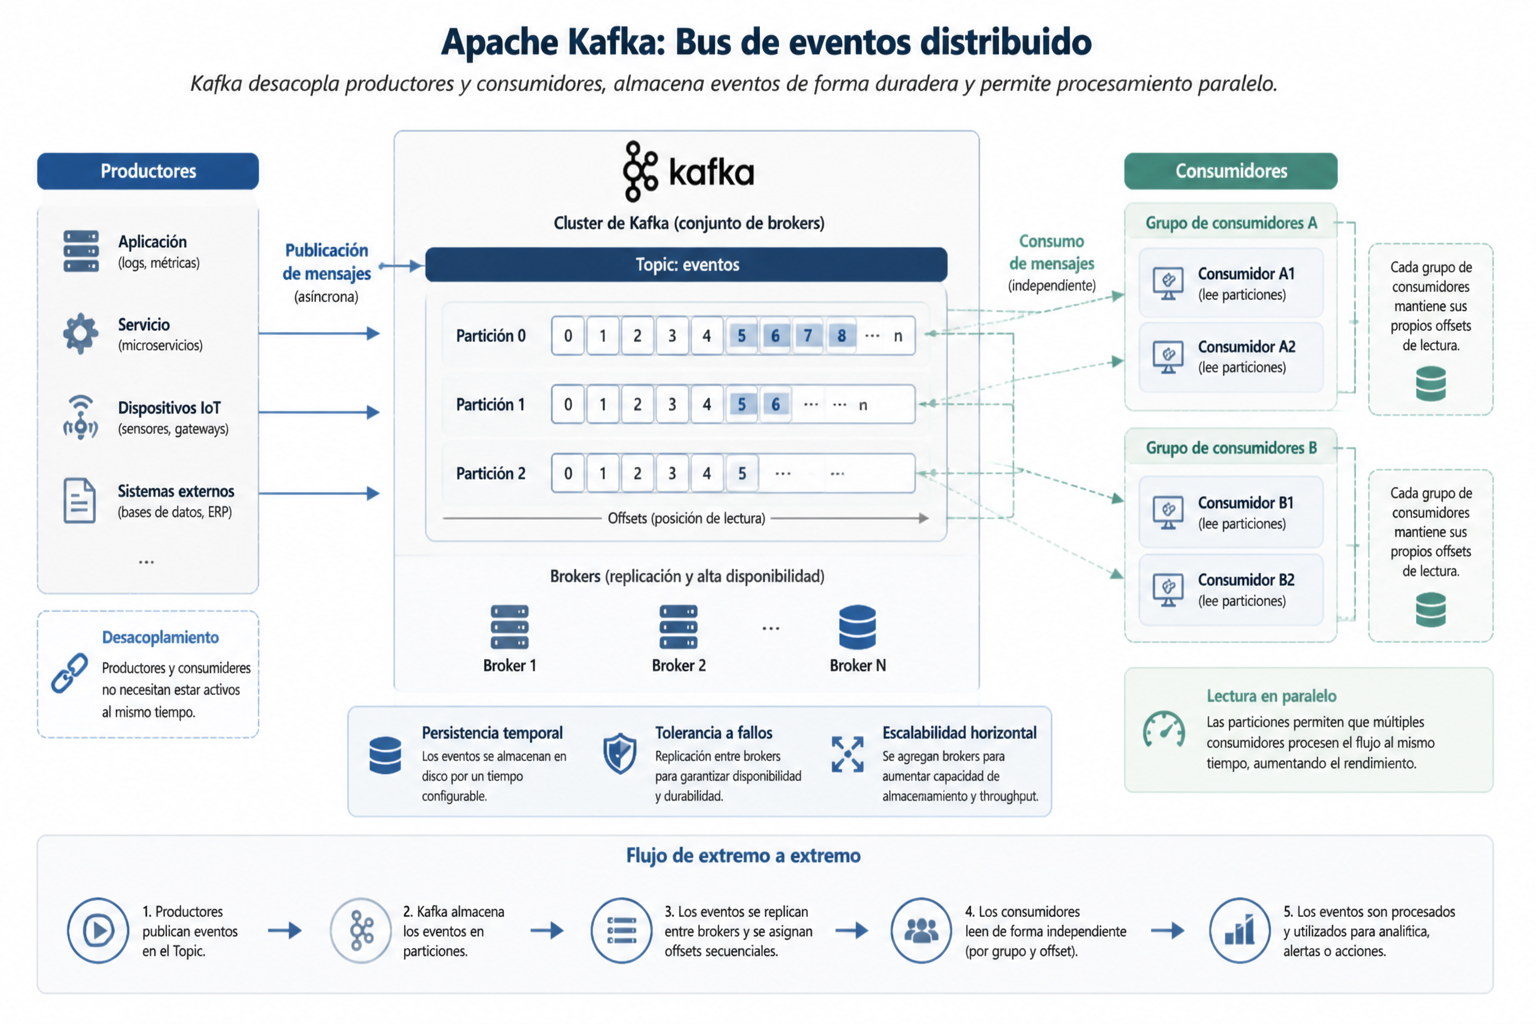
\includegraphics[width=\textwidth]{img/08.png}
    \column{0.44\textwidth}
      \begin{itemize}
        \item Organiza datos en \textit{topics} y particiones.
        \item Permite paralelismo, persistencia temporal y reprocesamiento.
        \item Varios consumidores pueden leer el mismo flujo para fines distintos.
      \end{itemize}
  \end{columns}
\end{frame}

\begin{frame}{Flink, Structured Streaming y Redis}
  \small
  \begin{tabularx}{\textwidth}{>{\RaggedRight\arraybackslash}p{3cm}X}
    \toprule
    \textbf{Tecnologia} & \textbf{Aporte principal} \\
    \midrule
    Flink & Motor orientado a estado, tiempo de evento, \textit{checkpoints} y baja latencia \\
    Structured Streaming & Streaming con DataFrames y SQL dentro del ecosistema Spark \\
    Redis & Respuesta en milisegundos para rankings, sesiones, contadores y dashboards \\
    \bottomrule
  \end{tabularx}
  \vspace{0.25cm}
  \begin{block}{Lectura conjunta}
    Flume y Kafka mueven el dato; Flink y Structured Streaming lo procesan; Redis acerca el resultado a la aplicacion o al tablero.
  \end{block}
\end{frame}

\section{Casos de Uso}

\begin{frame}[plain]
  \centering
  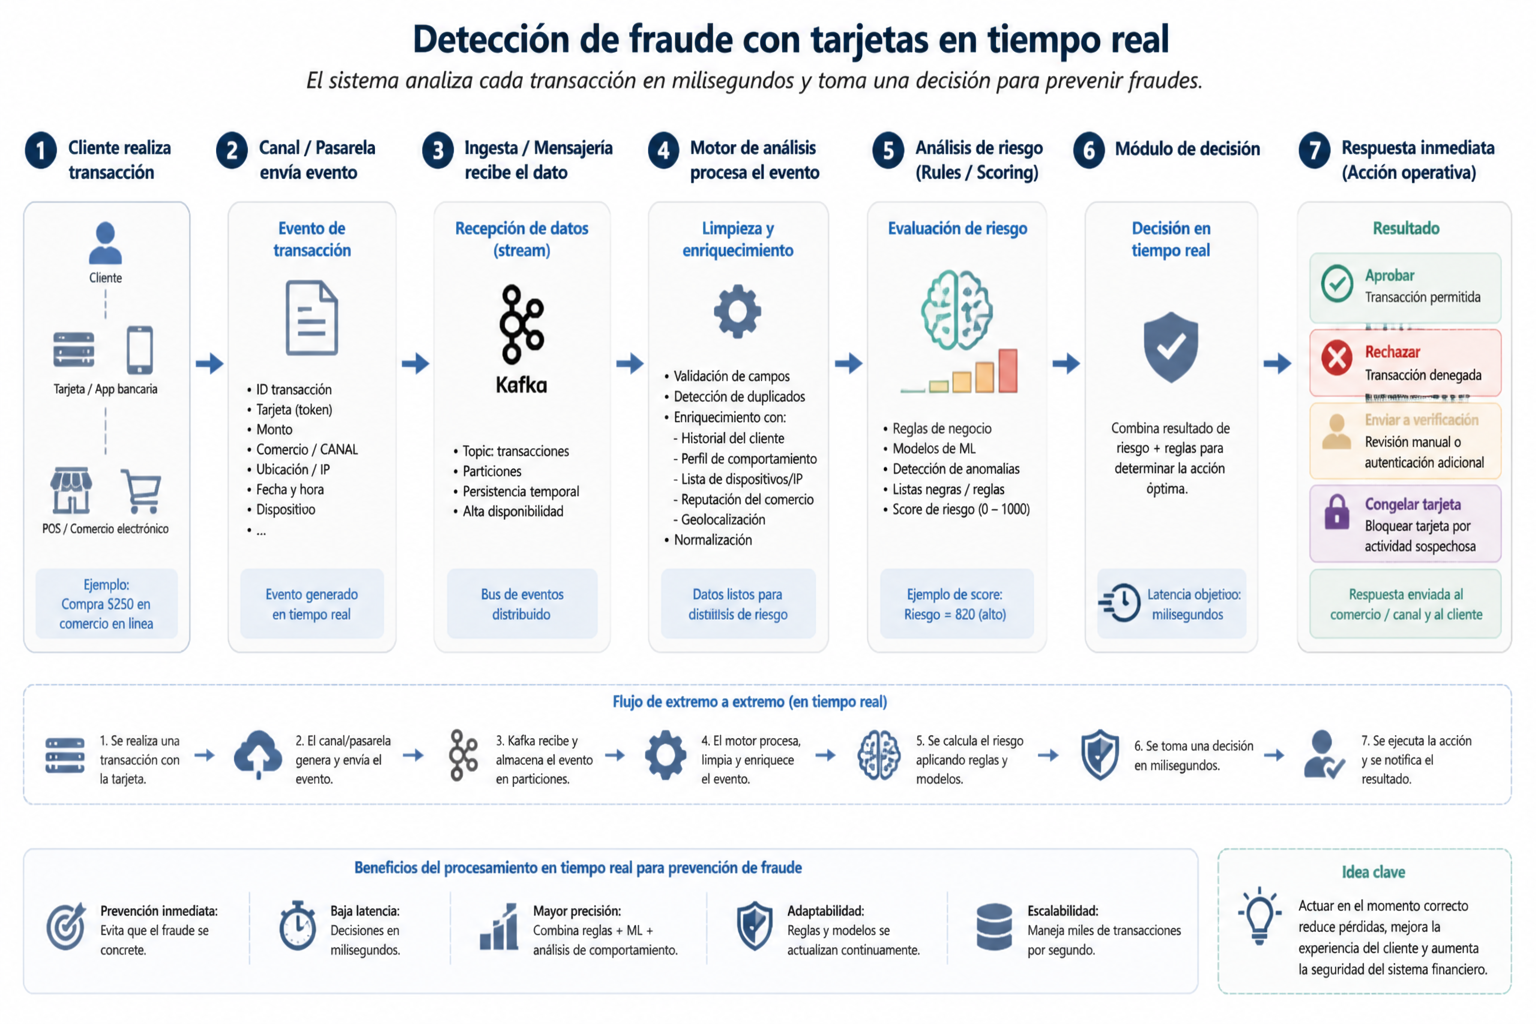
\includegraphics[width=\paperwidth,height=0.9\paperheight,keepaspectratio]{img/09.png}
\end{frame}

\begin{frame}{Lectura del caso de fraude}
  \begin{itemize}
    \item El evento se analiza mientras la transaccion aun esta en curso.
    \item La salida puede ser aprobar, rechazar, verificar o congelar la tarjeta.
    \item Aqui la latencia impacta directamente en el riesgo economico.
    \item Este caso resume bien el valor del procesamiento en tiempo real: actuar antes de que el daño se concrete.
  \end{itemize}
\end{frame}

\begin{frame}{Analitica e-commerce}
  \begin{columns}[T]
    \column{0.6\textwidth}
      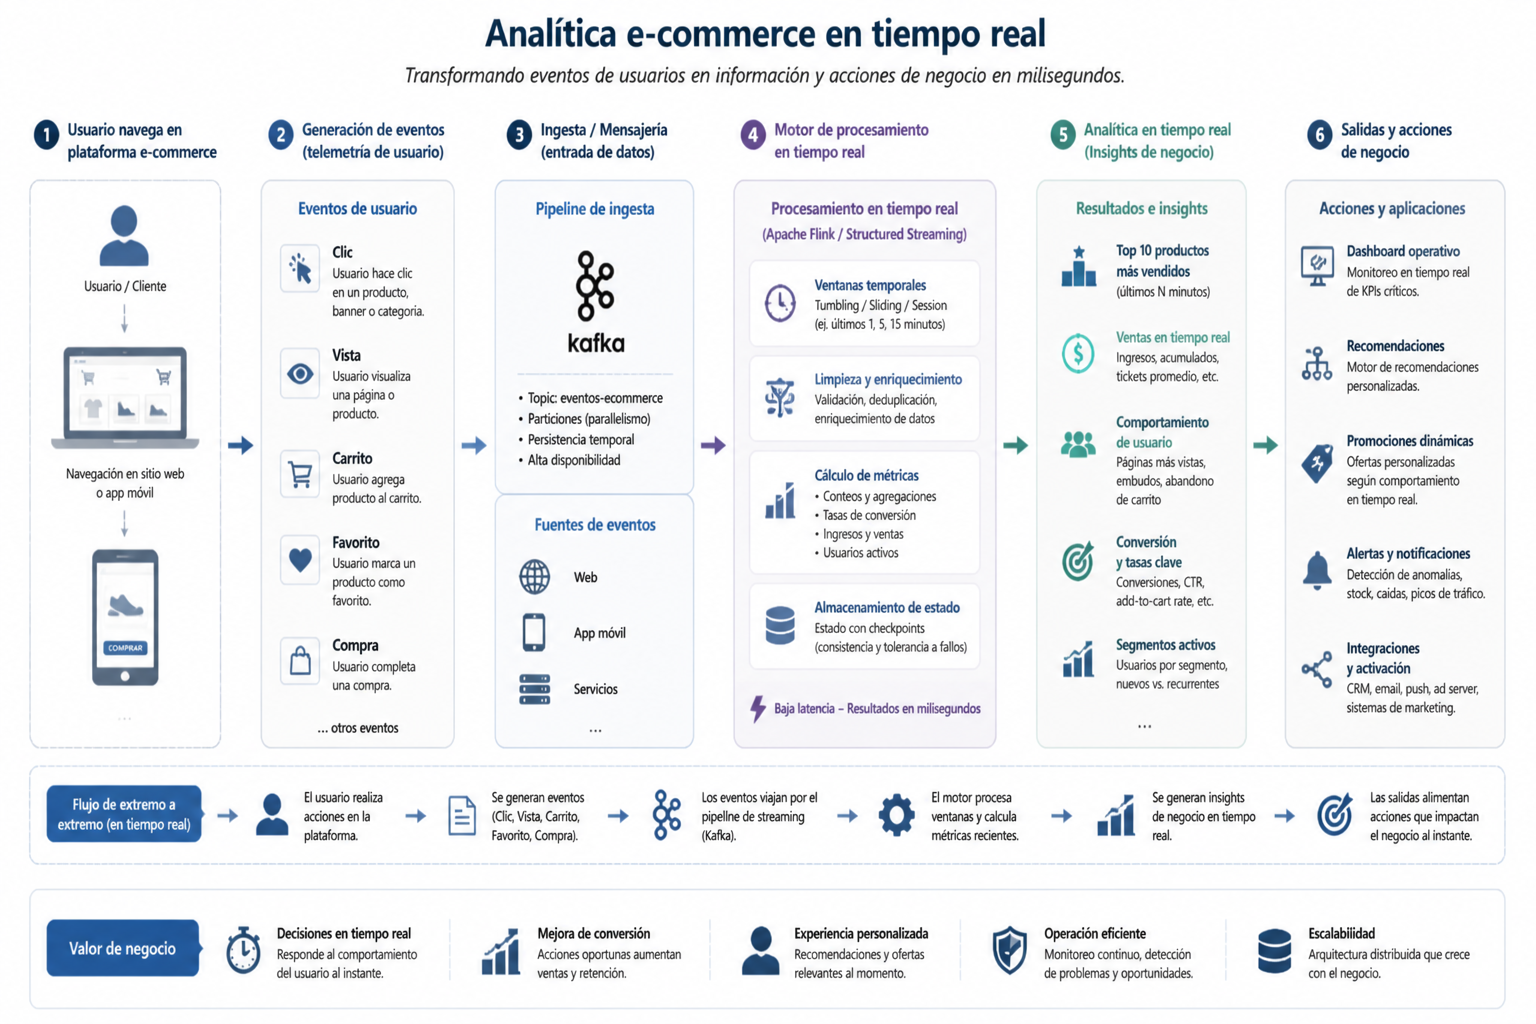
\includegraphics[width=\textwidth]{img/6-2-ecommerce.png}
    \column{0.4\textwidth}
      \begin{itemize}
        \item Eventos: clics, vistas, carrito, favoritos y compras.
        \item Se calculan rankings, top de productos y comportamiento reciente.
        \item La salida alimenta promociones, dashboards y recomendacion en tiempo real.
      \end{itemize}
  \end{columns}
\end{frame}

\begin{frame}{IoT y monitoreo}
  \begin{columns}[T]
    \column{0.6\textwidth}
      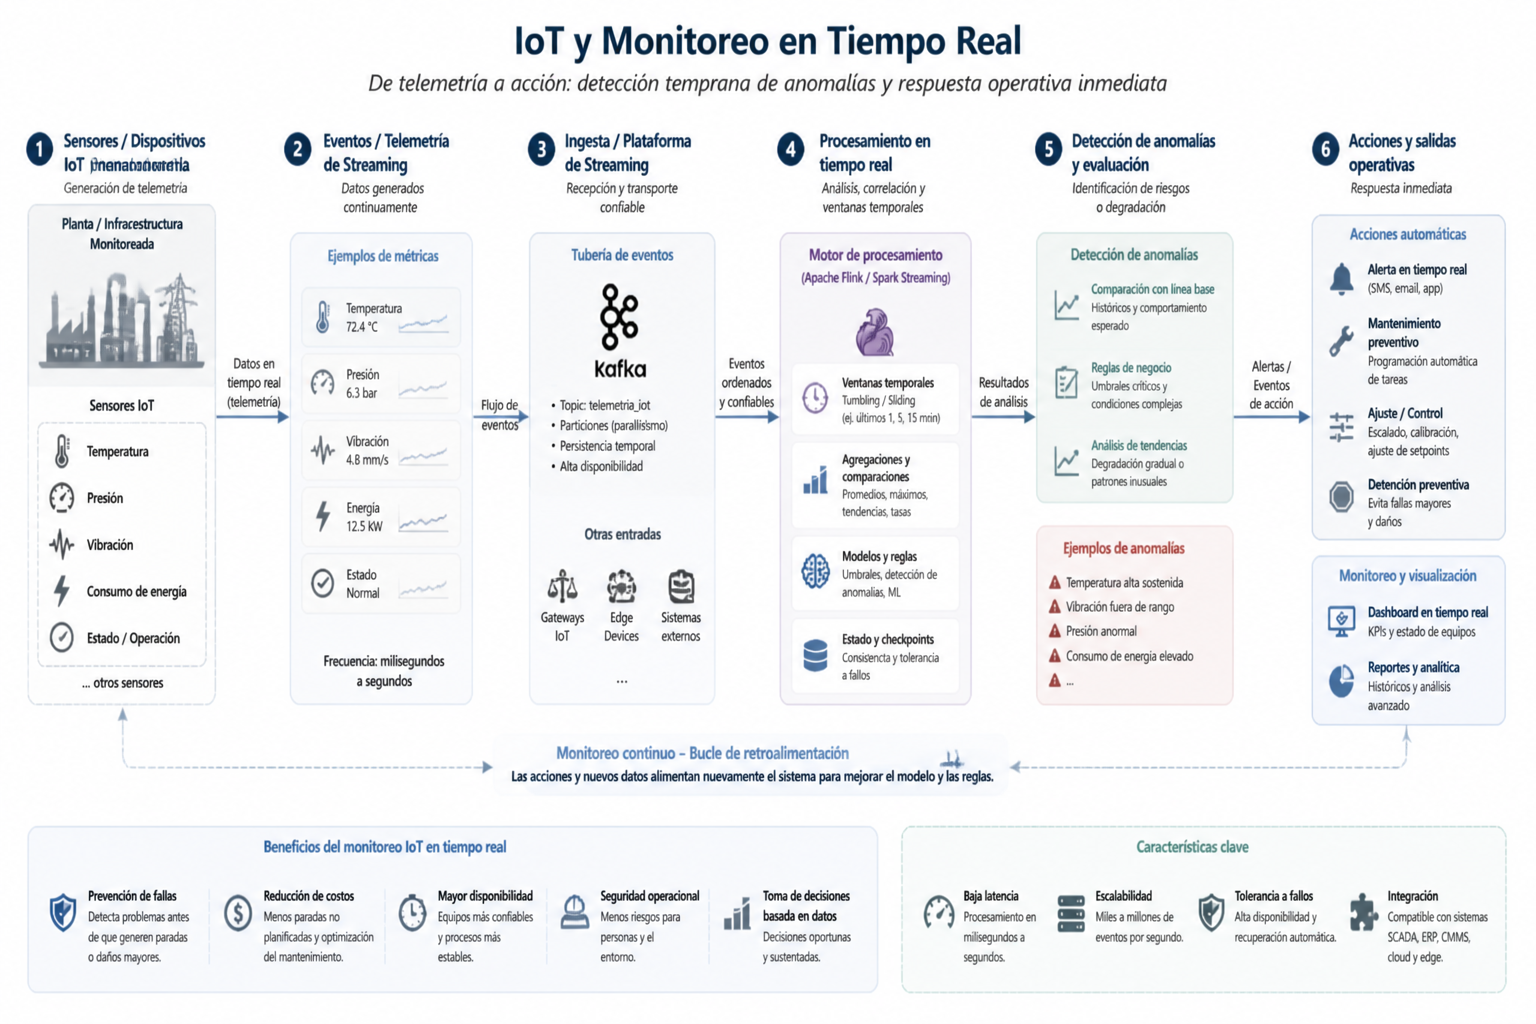
\includegraphics[width=\textwidth]{img/6-3-iot.png}
    \column{0.4\textwidth}
      \begin{itemize}
        \item Sensores envian telemetria continua: temperatura, presion, vibracion o consumo.
        \item El sistema detecta anomalias y activa alertas o mantenimiento preventivo.
        \item La baja latencia permite prevenir fallas antes de que escalen.
      \end{itemize}
  \end{columns}
\end{frame}

\begin{frame}{Ciberseguridad}
  \begin{columns}[T]
    \column{0.6\textwidth}
      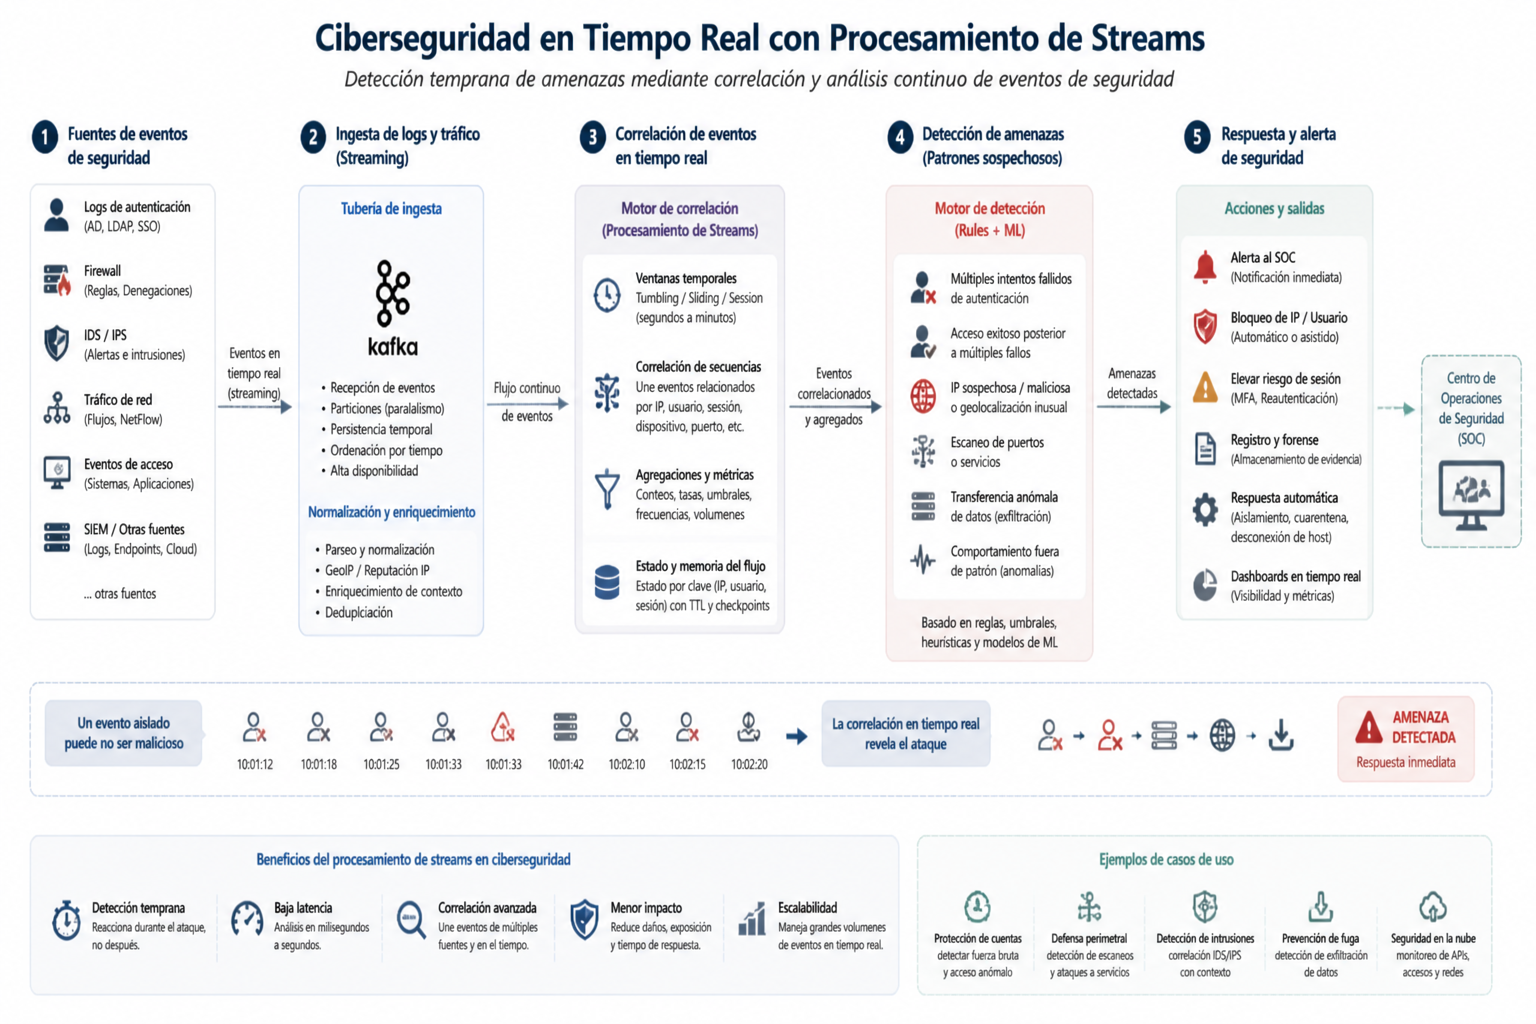
\includegraphics[width=\textwidth]{img/6-4-ciberseguridad.png}
    \column{0.4\textwidth}
      \begin{itemize}
        \item Se correlacionan logs, autenticaciones, firewall e IDS.
        \item El valor no esta en mirar un evento aislado, sino una secuencia sospechosa.
        \item La respuesta puede ser alerta, bloqueo o elevacion de riesgo.
      \end{itemize}
  \end{columns}
\end{frame}

\section{Vigencia}

\begin{frame}{Vigencia y evolucion del ecosistema}
  \begin{itemize}
    \item \textbf{Kafka}: evolucion hacia KRaft y menor dependencia operativa externa.
    \item \textbf{Flink}: mayor madurez en SQL, conectores, Kubernetes y manejo de estado.
    \item \textbf{Structured Streaming}: integracion fuerte con Spark 3.x y Delta Lake.
    \item El ecosistema actual incluye alternativas como Pulsar, Kinesis o Pub/Sub.
    \item Los principios del capitulo siguen vigentes: latencia, throughput, desacoplamiento, estado y tolerancia a fallos.
  \end{itemize}
\end{frame}

\section{Laboratorio}

\begin{frame}{Laboratorio propuesto}
  \begin{block}{Caso elegido}
    Deteccion de fraude con tarjetas en tiempo real.
  \end{block}
  \begin{itemize}
    \item \textbf{Entrada}: transacciones JSON con \textit{event time} y \textit{arrival time}.
    \item \textbf{Flujo}: fuente, broker simulado, procesador y sink de decisiones.
    \item \textbf{Salida}: consola, checkpoints y dashboard web local.
    \item \textbf{Objetivo}: mostrar ventanas, estado, \textit{watermarks}, eventos tardios y deduplicacion.
  \end{itemize}
\end{frame}

\begin{frame}{Flujo del laboratorio}
  \centering
  \begin{tikzpicture}[node distance=0.7cm]
    \node[box] (src) {Fuente de\\transacciones};
    \node[box, right=of src] (broker) {Broker\\simulado};
    \node[box, right=of broker] (proc) {Motor de\\streaming};
    \node[box, right=of proc] (sink) {Sink de\\decisiones};
    \node[smallbox, below=of proc] (ckpt) {Checkpoints};
    \node[smallbox, above=of sink] (dash) {Dashboard\\web};

    \draw[line] (src) -- (broker);
    \draw[line] (broker) -- (proc);
    \draw[line] (proc) -- (sink);
    \draw[line] (proc) -- (ckpt);
    \draw[line] (sink) -- (dash);
  \end{tikzpicture}
  \vspace{0.25cm}

  \begin{itemize}
    \item El flujo reproduce la logica del capitulo aunque la demo corra localmente en Python.
    \item Lo importante es observar como el evento entra, se contextualiza y termina en una decision operativa.
  \end{itemize}
\end{frame}

\begin{frame}{Que demuestra la demo}
  \begin{itemize}
    \item \textbf{Event time vs processing time}: se procesa por orden de llegada, pero se decide usando tiempo de evento.
    \item \textbf{Ventanas y estado}: el sistema conserva historial reciente por tarjeta.
    \item \textbf{Watermarks}: detecta eventos demasiado tardios respecto al flujo observado.
    \item \textbf{Deduplicacion}: ignora un \textit{event\_id} repetido.
    \item \textbf{Decisiones}: `APROBAR`, `REVISAR`, `BLOQUEAR`, `AUDITAR\_TARDE` e `IGNORAR\_DUPLICADO`.
  \end{itemize}
\end{frame}

\begin{frame}{Como se expone el laboratorio}
  \begin{enumerate}
    \item Mostrar el archivo de transacciones y explicar sus campos.
    \item Abrir el dashboard en el navegador y lanzar la simulacion.
    \item Seguir visualmente el paso por fuente, broker, procesador y sink.
    \item Resaltar el evento tardio, el duplicado y el caso bloqueado.
    \item Cerrar mostrando los checkpoints como ejemplo de recuperacion de estado.
  \end{enumerate}
\end{frame}

\section{Cierre}

\begin{frame}{Conclusiones}
  \begin{itemize}
    \item El \textit{stream processing} permite actuar antes de que el dato pierda valor.
    \item La arquitectura combina ingesta, mensajeria, computo y salida operativa.
    \item Flume, Kafka, Flink, Structured Streaming y Redis cumplen roles complementarios.
    \item Los casos de fraude, e-commerce, IoT y ciberseguridad muestran su impacto real.
    \item El tema es suficientemente solido para construir monografia, presentacion y laboratorio.
  \end{itemize}
\end{frame}

\begin{frame}{Referencias base}
  \small
  \begin{itemize}
    \item Huawei Technologies Co., Ltd. \textit{HCIP Big Data Developer V2.0 Training Material}, 2022.
    \item Apache Kafka Documentation.
    \item Apache Flink Documentation.
    \item Apache Spark Structured Streaming Programming Guide.
    \item Redis Documentation.
  \end{itemize}
\end{frame}

\end{document}
